\documentclass[UTF8,a4paper,12pt]{ctexart}

\usepackage{geometry}
\usepackage{graphicx}
\usepackage{float}
\usepackage{listings}
\usepackage{xcolor}
\usepackage{setspace}

\usepackage[hidelinks]{hyperref}
\usepackage{enumitem}
\usepackage{amsmath}

\geometry{
left=2.5cm,
right=2.5cm,
top=2.5cm,
bottom=2.5cm
}

\setstretch{1.35}

\lstset{
basicstyle=\ttfamily\small,
breaklines=true,
frame=single,
numbers=left,
numberstyle=\tiny,
tabsize=4,
showstringspaces=false
}

\begin{document}

\begin{titlepage}
\centering
\begin{figure}
    \centering
    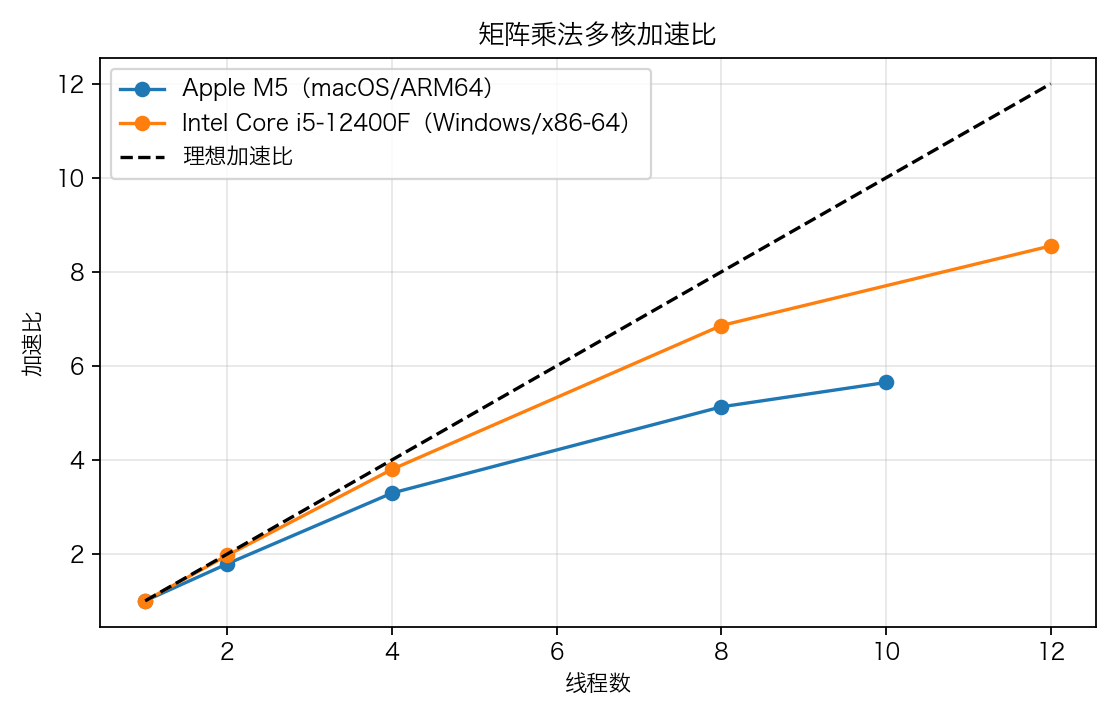
\includegraphics[width=0.8\linewidth]{results/comparison/figures/multicore_speedup.png}
\end{figure}
\vspace*{2cm}

{\zihao{2}\heiti 计算机体系结构系统性能评价实验报告\par}

\vspace{2cm}

{\zihao{3}\heiti 实验选题：\par}
\vspace{0.5cm}
{\zihao{3}\heiti Apple M5 与 Intel Core i5-12400F 的 CPU 性能对比\par}

\vspace{2cm}

\begin{center}
\zihao{4}
姓名：\underline{\makebox[8cm][c]{宋杲行}} \\[0.5cm]
学号：\underline{\makebox[8cm][c]{24281073}} \\[0.5cm]
指导教师：\underline{\makebox[8cm][c]{赵宏智}} \\[0.5cm]
完成日期：\underline{\makebox[8cm][c]{2026/09/14}} \\[0.5cm]
仓库地址：\underline{\makebox[13cm][c]{https://github.com/Hanggoash/Lab1}} \\[0.5cm]
\end{center}
\vfill

\begin{flushleft}
\textbf{自我评价：}

\hspace{2em}本次实验完成了同一套 C++17 CPU Toy Benchmark 在 Apple M5 与 Intel Core i5-12400F 真机上的构建、运行和数据汇总，并使用 Cinebench 2026 补充 CPU 渲染场景测试。实验保留了逐次原始数据和编译元数据，围绕单线程、多线程、缓存/内存访问三个维度分析结果，并结合阿姆达尔定律和 CPU 性能公式解释性能差异及其边界。
\end{flushleft}

\vspace{1cm}

\vspace{1cm}

{\zihao{4}北京交通大学计算机科学与技术学院\par}

\end{titlepage}

\tableofcontents
\newpage

\section{实验目的}

本实验对比两台真实设备上的 CPU 性能：Apple M5（macOS / ARM64）和 Intel Core i5-12400F（Windows / x86-64）。实验以自建 CPU Toy Benchmark 为主要评价工具，并以 Cinebench 2026 的 CPU 渲染分数作为补充。两类测试的侧重点不同：Toy Benchmark 将问题拆分为整数循环、分支与排序、矩阵计算、多线程扩展以及顺序/随机内存访问；Cinebench 则考察实际三维渲染工作负载下的单线程和多线程 CPU 吞吐。

实验目标如下：

\begin{enumerate}
\item 在两台设备上运行相同的 C++17 源代码、算法、输入规模和随机种子，获得可追溯的 CPU 实测数据。
\item 通过筛法、快速排序、普通矩阵乘法、多线程矩阵乘法和内存访问测试，从多个维度评价 CPU 性能。
\item 对 Toy Benchmark 的每个配置进行 10 次正式重复，计算均值、样本标准差、最小值和最大值，避免以单次结果替代统计结果。
\item 使用 Cinebench 2026.1.3 的单线程和多线程 CPU 测试补充真实渲染场景；该部分按单次正式测试记录，作为趋势验证而非重复性统计。
\item 结合 CPU 性能公式、阿姆达尔定律、核心/线程组织和存储访问局部性，解释不同工作负载下的性能差异。
\item 在实验边界内形成面向学习、开发和 CPU 渲染场景的硬件选择建议，而不泛化为 ARM 或 x86 指令集的普遍优劣。
\end{enumerate}

\section{实验环境与测试方法}

\subsection{硬件与软件环境}

表\ref{tab:environment}列出两台设备及其实际测试环境。Windows 端的 CPU 型号由设备界面人工确认；其 Toy Benchmark 元数据中 CPU 自动识别字段为 unavailable，因此报告中不将该字段误写为自动识别结果。

\begin{table}[H]
    \centering
    \renewcommand{\arraystretch}{1.35}
    \caption{实验环境}
    \label{tab:environment}
    \small
    \begin{tabular}{p{3.0cm} p{5.0cm} p{5.0cm}}
        \hline
        项目 & Apple M5 平台 & Intel 平台 \\
        \hline
        CPU & Apple M5 & Intel Core i5-12400F \\
        操作系统与架构 & macOS 26.5（25F71），ARM64 & Windows 11 64 Bit（build 26200），x86-64 \\
        核心/线程信息 & 测试程序检测到 10 个硬件并发线程 & 6 核、12 线程 \\
        Toy Benchmark 编译器 & AppleClang 21.0.0.21000101 & GNU 16.1.0 \\
        语言与构建类型 & C++17，Release & C++17，Release \\
        基线编译选项 & \texttt{-O2 -fno-vectorize -fno-slp-vectorize -fno-unroll-loops -fno-fast-math} & \texttt{-O2 -fno-tree-vectorize -fno-tree-slp-vectorize -fno-unroll-loops -fno-fast-math} \\
        Cinebench 版本 & Cinebench 2026.1.3 & Cinebench 2026.1.3 \\
        \hline
    \end{tabular}
\end{table}

两端均未主动使用 \texttt{-march=native}、\texttt{-mcpu=native}、LTO、PGO、fast-math、手写 NEON/AVX 指令、BLAS、GPU 或硬件性能计数器。两端最终机器指令因 ARM64、x86-64、操作系统和编译器不同而不可能完全一致；本实验比较的是同一高级语言 workload 在这两个实际平台上的最终表现。

\subsection{Toy Benchmark 设计与公平性控制}

自建测试只依赖 C++ 标准库，使用 \texttt{std::chrono::steady\_clock} 计时。所有随机输入均使用固定种子 \texttt{std::mt19937(12345)}；初始化、随机数生成、输入复制、正确性校验、CSV 写入和日志均不计入核心执行时间。每项测试先预热 1 次，再正式运行 10 次；每次正式运行在 raw CSV 中各占一行，并配套保存 JSON 元数据。

测试项目及其主要观测维度如下：

\begin{itemize}
\item 埃拉托斯特尼筛法：整数运算、循环和数组访问；规模为 1M、5M、10M、50M。
\item Hoare 快速排序：比较、分支、交换和缓存访问；规模为 100K、1M、5M、10M 个元素。
\item 普通三重循环矩阵乘法：单线程计算时间和 GFLOPS；矩阵维度为 128、256、512、1024。
\item 多线程矩阵乘法：在 $N=512$ 下使用 \texttt{std::thread} 划分行任务，记录不同线程数下的时间、加速比和并行效率。
\item 顺序/随机内存访问：工作集为 32 KiB 至 256 MiB；随机索引在计时前生成，指标为每秒百万次有效访问，不将其误称为硬件带宽。
\end{itemize}

相对性能统一定义为：

\[
\mathrm{Speedup}_{M5} = \frac{T_{\mathrm{i5\text{-}12400F}}}{T_{M5}}
\]

当该值大于 1 时，表示 M5 在该工作负载下用时更短；小于 1 则表示 i5-12400F 用时更短。不同单位（毫秒、GFLOPS、内存访问吞吐、Cinebench 分数）不进行算术平均或加权合成。

\subsection{Cinebench 测试方法}

Cinebench 仅测试 CPU 项目，不测试 GPU。两台设备均使用 Cinebench 2026.1.3，分别记录 \texttt{CPU (Single Thread)} 与 \texttt{CPU (Multiple Threads)} 的 1 次正式分数，并由软件给出：

\[
\mathrm{MP\ Ratio}=\frac{\mathrm{CPU\ (Multiple\ Threads)\ score}}{\mathrm{CPU\ (Single\ Thread)\ score}}
\]

由于 Cinebench 每个项目只保留一次正式结果，本报告不为其计算均值或标准差，也不将其与 Toy Benchmark 的 10 次统计结果混为同一精度等级。测试时关闭无关程序，使用同一版本软件，并记录结果界面截图作为证据。

\section{Toy Benchmark 实验结果}

本节时间均为 10 次正式运行的均值 $\pm$ 样本标准差。完整原始 CSV、元数据和全部汇总结果均提交在仓库的 \texttt{results/} 目录中；表格数据可追溯到每一条正式运行记录。

\subsection{筛法与快速排序}

筛法反映整数循环和连续数组标记的基础执行能力，快速排序则额外包含大量比较、分支、交换和非连续访问。表\ref{tab:sieve}和表\ref{tab:quicksort}给出全部规模的结果。

\begin{table}[H]
    \centering
    \renewcommand{\arraystretch}{1.35}
    \caption{埃拉托斯特尼筛法结果}
    \label{tab:sieve}
    \begin{tabular}{c c c c}
        \hline
        问题规模 & M5 时间（ms） & i5-12400F 时间（ms） & M5 相对性能 \\
        \hline
        1,000,000 & $1.109 \pm 0.062$ & $0.940 \pm 0.062$ & $0.847\times$ \\
        5,000,000 & $4.914 \pm 0.392$ & $9.657 \pm 0.330$ & $1.965\times$ \\
        10,000,000 & $9.383 \pm 0.337$ & $21.192 \pm 0.533$ & $2.258\times$ \\
        50,000,000 & $122.813 \pm 2.102$ & $250.455 \pm 11.872$ & $2.039\times$ \\
        \hline
    \end{tabular}
\end{table}

当规模为 1M 时，两端绝对时间约为 1 ms，计时固定开销和短时调度扰动的影响相对更明显，i5-12400F 略快。规模增大后，M5 的时间明显更短，在 5M、10M、50M 下相对性能分别为 $1.965\times$、$2.258\times$ 和 $2.039\times$。因此不能以最小规模的单点结果代表更长的整数循环任务。

\begin{figure}[H]
    \centering
    \fbox{%
        \begin{minipage}[c][6cm][c]{12cm}
            \centering
            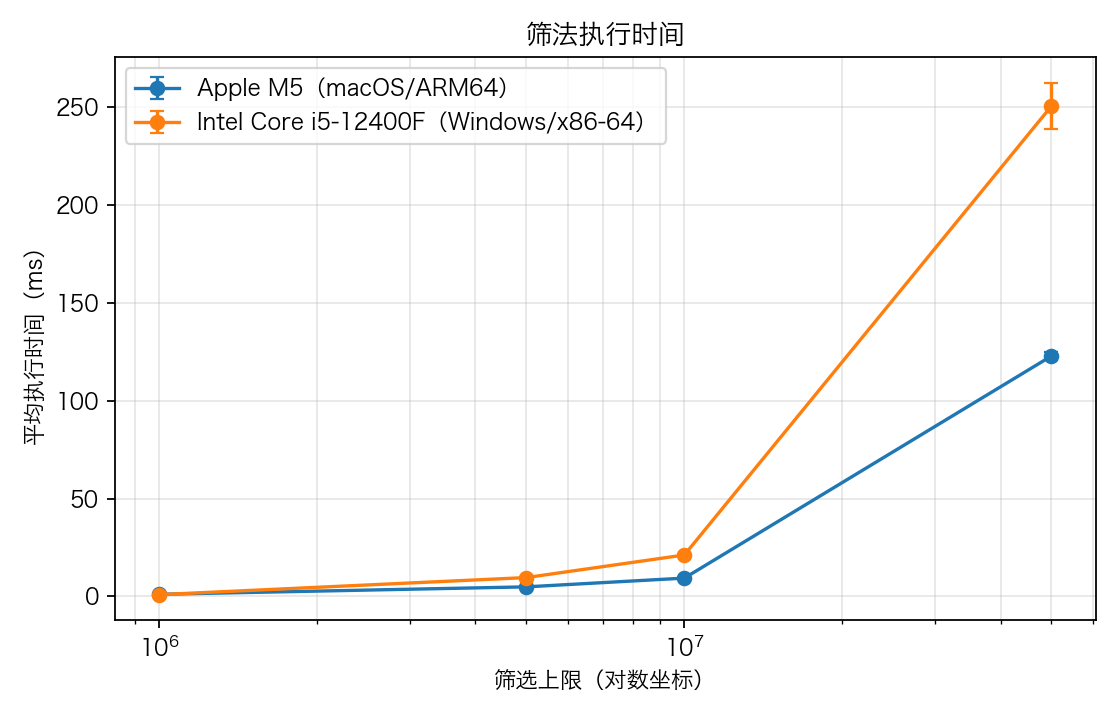
\includegraphics[width=\linewidth,height=6cm,keepaspectratio]{results/comparison/figures/sieve_comparison.png}
        \end{minipage}
    }
    \caption{筛法平均执行时间对比}
\end{figure}

\begin{table}[H]
    \centering
    \renewcommand{\arraystretch}{1.35}
    \caption{Hoare 快速排序结果}
    \label{tab:quicksort}
    \begin{tabular}{c c c c}
        \hline
        元素数量 & M5 时间（ms） & i5-12400F 时间（ms） & M5 相对性能 \\
        \hline
        100,000 & $4.078 \pm 0.140$ & $6.405 \pm 0.163$ & $1.570\times$ \\
        1,000,000 & $47.558 \pm 1.025$ & $72.045 \pm 0.631$ & $1.515\times$ \\
        5,000,000 & $247.479 \pm 1.638$ & $391.665 \pm 8.625$ & $1.583\times$ \\
        10,000,000 & $523.909 \pm 6.717$ & $827.498 \pm 17.696$ & $1.579\times$ \\
        \hline
    \end{tabular}
\end{table}

在四个快速排序规模下，M5 相对性能稳定在 $1.515\times$ 至 $1.583\times$。这一稳定差距说明，在本实现的比较、分支、交换与缓存访问组合中，M5 的整体执行时间更短；但该结果仅适用于本项目的 Hoare 快速排序实现和固定输入，不代表所有排序程序。

\begin{figure}[H]
    \centering
    \fbox{%
        \begin{minipage}[c][6cm][c]{12cm}
            \centering
            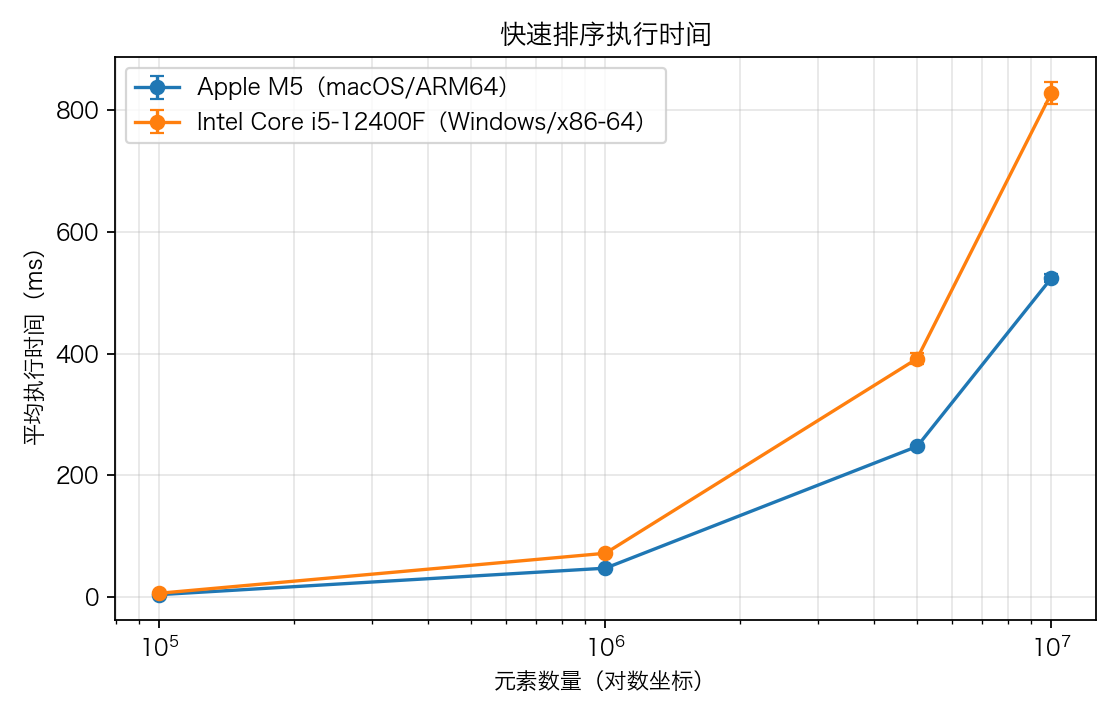
\includegraphics[width=\linewidth,height=6cm,keepaspectratio]{results/comparison/figures/quicksort_comparison.png}
        \end{minipage}
    }
    \caption{快速排序平均执行时间对比}
\end{figure}

\subsection{单线程矩阵乘法}

矩阵乘法固定采用普通 $i \rightarrow j \rightarrow k$ 三重循环，不调用 BLAS、Accelerate、MKL 或 SIMD intrinsic。GFLOPS 根据 $2N^3/T$ 由计时结果计算，因而仅描述本实现的有效计算吞吐。

\begin{table}[H]
    \centering
    \renewcommand{\arraystretch}{1.32}
    \caption{单线程矩阵乘法结果}
    \label{tab:matrix-single}
    \small
    \begin{tabular}{c c c c c c}
        \hline
        $N$ & M5 时间（ms） & i5 时间（ms） & M5 GFLOPS & i5 GFLOPS & M5 相对性能 \\
        \hline
        128 & $1.020 \pm 0.036$ & $1.106 \pm 0.126$ & $4.116 \pm 0.144$ & $3.829 \pm 0.371$ & $1.085\times$ \\
        256 & $9.785 \pm 0.086$ & $8.998 \pm 0.234$ & $3.429 \pm 0.030$ & $3.731 \pm 0.096$ & $0.920\times$ \\
        512 & $132.649 \pm 0.465$ & $295.206 \pm 3.415$ & $2.024 \pm 0.007$ & $0.909 \pm 0.011$ & $2.225\times$ \\
        1024 & $1193.008 \pm 9.790$ & $2810.930 \pm 107.188$ & $1.800 \pm 0.015$ & $0.765 \pm 0.027$ & $2.356\times$ \\
        \hline
    \end{tabular}
\end{table}

小矩阵下两端差距不稳定：$N=128$ 时 M5 略快，$N=256$ 时 i5 略快。矩阵扩大到 $N=512$、$N=1024$ 后，M5 相对性能上升至 $2.225\times$ 和 $2.356\times$。该普通循环对 B 矩阵的列访问局部性较差，结果同时受到计算流水线、缓存层次和内存访问行为影响，不能只用主频解释。

\begin{figure}[H]
    \centering
    \fbox{%
        \begin{minipage}[c][6cm][c]{12cm}
            \centering
            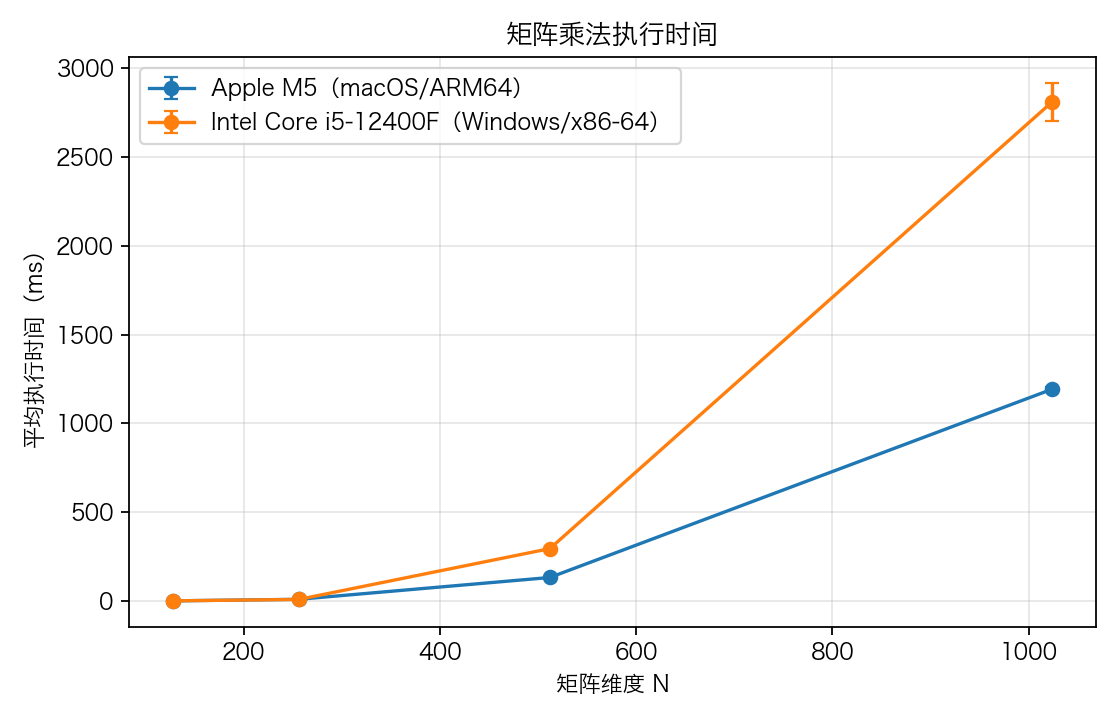
\includegraphics[width=\linewidth,height=6cm,keepaspectratio]{results/comparison/figures/matrix_execution_time.png}
        \end{minipage}
    }
    \caption{单线程矩阵乘法执行时间对比}
\end{figure}

\begin{figure}[H]
    \centering
    \fbox{%
        \begin{minipage}[c][6cm][c]{12cm}
            \centering
            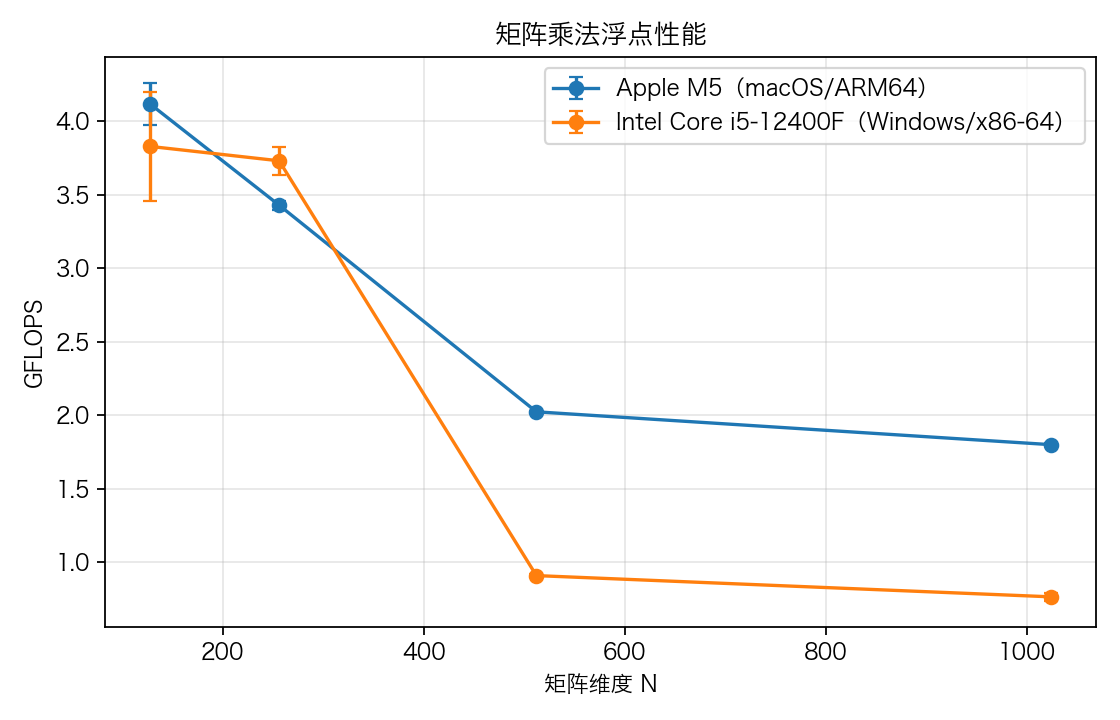
\includegraphics[width=\linewidth,height=6cm,keepaspectratio]{results/comparison/figures/matrix_gflops.png}
        \end{minipage}
    }
    \caption{单线程矩阵乘法 GFLOPS 对比}
\end{figure}

\subsection{多线程矩阵乘法}

多线程测试固定为 $N=512$。跨平台仅比较两端共有的 2、4、8 线程配置；M5 的硬件并发数为 10，i5-12400F 为 12，因此 10 与 12 线程点仅用于各自平台的本机扩展曲线，不能直接横向配对。

\begin{table}[H]
    \centering
    \renewcommand{\arraystretch}{1.32}
    \caption{多线程矩阵乘法（$N=512$）结果}
    \label{tab:matrix-multi}
    \small
    \begin{tabular}{c c c c c c}
        \hline
        线程数 & M5 时间（ms） & i5 时间（ms） & M5 加速比 & i5 加速比 & M5 相对性能 \\
        \hline
        2 & $74.082 \pm 4.480$ & $149.785 \pm 5.507$ & $1.791\times$ & $1.971\times$ & $2.022\times$ \\
        4 & $40.263 \pm 2.082$ & $77.701 \pm 1.558$ & $3.295\times$ & $3.799\times$ & $1.930\times$ \\
        8 & $25.866 \pm 0.713$ & $43.047 \pm 0.894$ & $5.128\times$ & $6.858\times$ & $1.664\times$ \\
        \hline
    \end{tabular}
\end{table}

在相同的 2、4、8 线程数下，M5 的绝对执行时间均更短，相对性能为 $1.664\times$ 至 $2.022\times$。但按各自单线程时间计算的本机加速比，i5-12400F 更接近理想线性扩展。这两个结论并不矛盾：前者比较总完成时间，后者比较同一设备由单线程到多线程的相对增益。

\begin{figure}[H]
    \centering
    \fbox{%
        \begin{minipage}[c][6cm][c]{12cm}
            \centering
            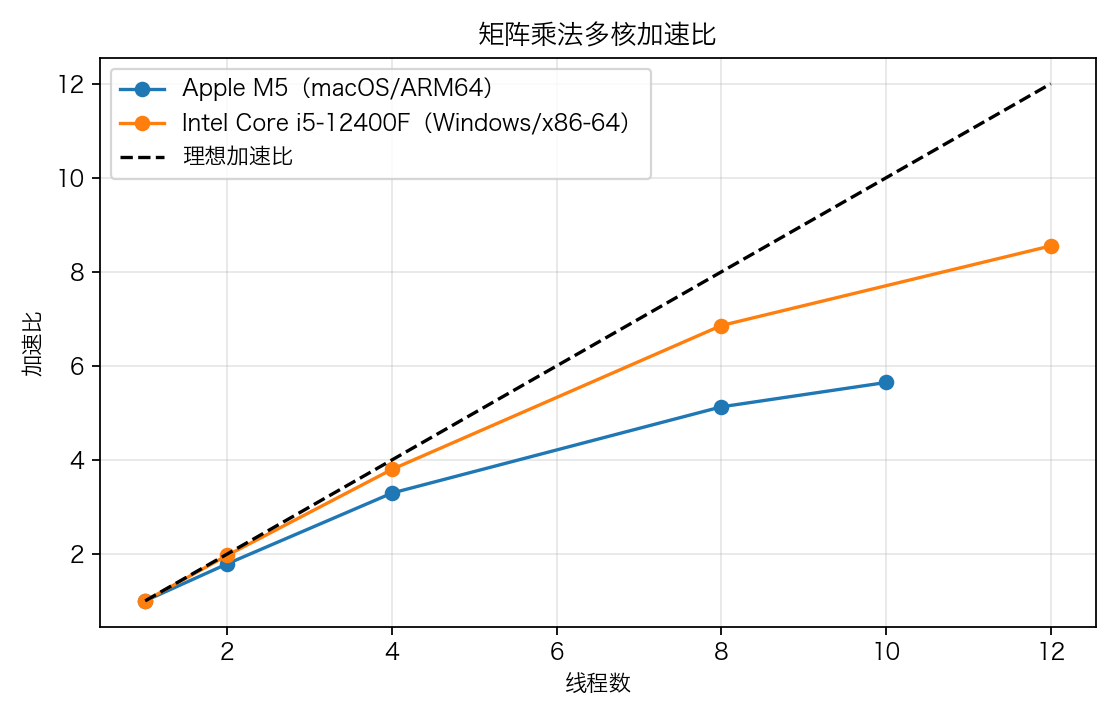
\includegraphics[width=\linewidth,height=6cm,keepaspectratio]{results/comparison/figures/multicore_speedup.png}
        \end{minipage}
    }
    \caption{多线程矩阵乘法加速比与理想线性加速对比}
\end{figure}

\begin{figure}[H]
    \centering
    \fbox{%
        \begin{minipage}[c][6cm][c]{12cm}
            \centering
            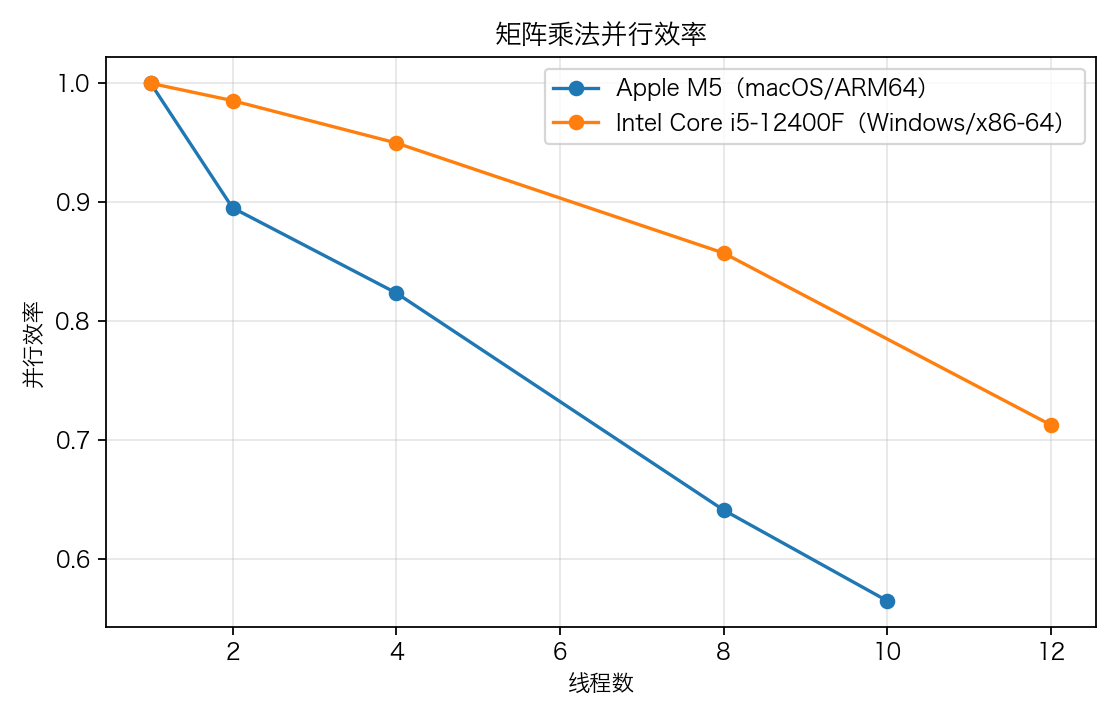
\includegraphics[width=\linewidth,height=6cm,keepaspectratio]{results/comparison/figures/parallel_efficiency.png}
        \end{minipage}
    }
    \caption{多线程矩阵乘法并行效率对比}
\end{figure}

\subsection{顺序与随机内存访问}

表\ref{tab:memory}列出若干代表性工作集，完整的 32 KiB 至 256 MiB 数据已保存在比较 CSV。顺序访问在较小工作集上两端接近，随着工作集增大，M5 在 16 MiB 至 256 MiB 的吞吐高于 i5。随机访问对局部性更敏感：在 16 MiB 工作集下，M5 为 $1350.830$ 百万次访问/秒，i5 为 $332.208$ 百万次访问/秒，M5 相对性能为 $4.035\times$；但 256 KiB 下 i5 略快。这表明工作集大小和访问模式会显著改变结果，不能将某一工作集的结论外推到所有内存任务。

\begin{table}[H]
    \centering
    \renewcommand{\arraystretch}{1.3}
    \caption{代表性内存访问吞吐（百万次访问/秒）}
    \label{tab:memory}
    \small
    \begin{tabular}{c c c c c}
        \hline
        模式 & 工作集 & M5 & i5-12400F & M5 相对性能 \\
        \hline
        顺序 & 32 KiB & $3895.575 \pm 127.204$ & $3960.877 \pm 65.151$ & $0.983\times$ \\
        顺序 & 4 MiB & $4235.501 \pm 68.198$ & $3970.613 \pm 369.858$ & $1.076\times$ \\
        顺序 & 16 MiB & $4117.128 \pm 191.516$ & $3482.973 \pm 390.698$ & $1.195\times$ \\
        顺序 & 256 MiB & $4158.768 \pm 45.688$ & $3501.085 \pm 48.350$ & $1.188\times$ \\
        随机 & 256 KiB & $2392.530 \pm 54.032$ & $2528.953 \pm 284.174$ & $0.958\times$ \\
        随机 & 4 MiB & $1781.199 \pm 25.883$ & $751.641 \pm 34.364$ & $2.374\times$ \\
        随机 & 16 MiB & $1350.830 \pm 135.294$ & $332.208 \pm 12.606$ & $4.035\times$ \\
        随机 & 256 MiB & $336.517 \pm 0.294$ & $131.654 \pm 0.722$ & $2.556\times$ \\
        \hline
    \end{tabular}
\end{table}

\begin{figure}[H]
    \centering
    \fbox{%
        \begin{minipage}[c][6cm][c]{12cm}
            \centering
            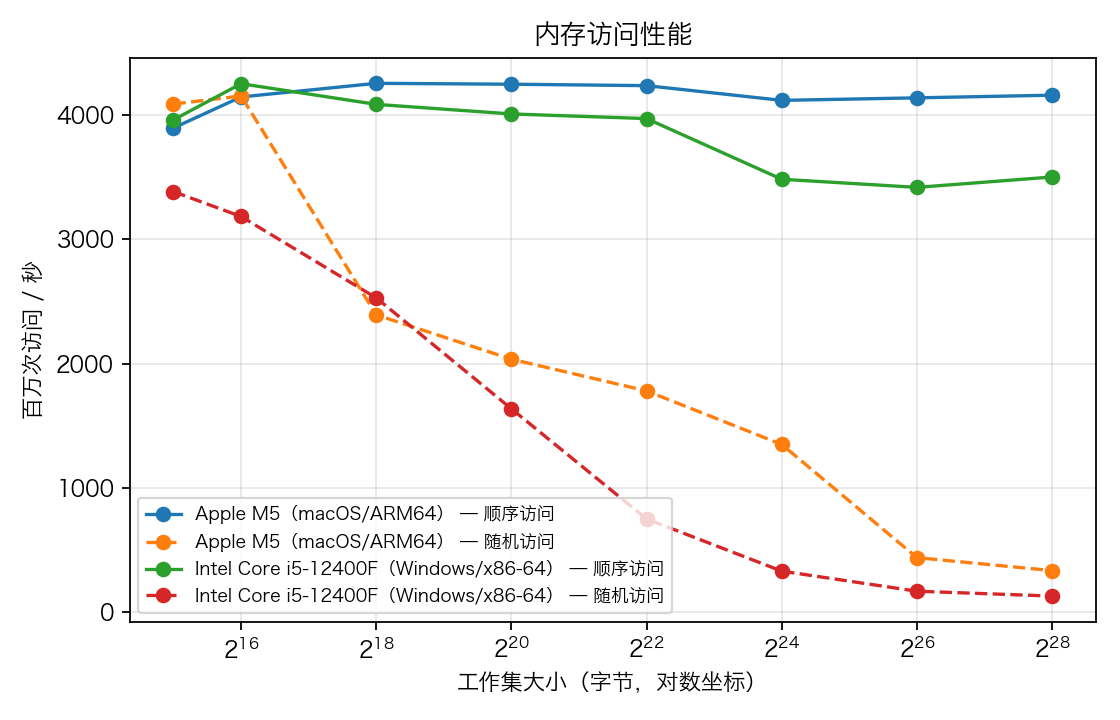
\includegraphics[width=\linewidth,height=6cm,keepaspectratio]{results/comparison/figures/memory_performance.png}
        \end{minipage}
    }
    \caption{顺序与随机内存访问性能对比}
\end{figure}

\section{Cinebench 2026 实验结果}

\subsection{单线程、多线程分数与 MP Ratio}

表\ref{tab:cinebench}为 Cinebench 2026.1.3 的单次正式 CPU 测试结果。该软件的分数越高表示性能越高，与 Toy Benchmark 的“时间越短越好”方向相反。MP Ratio 由同一设备的多线程分数除以单线程分数得到。

\begin{table}[H]
    \centering
    \renewcommand{\arraystretch}{1.4}
    \caption{Cinebench 2026.1.3 CPU 单次正式结果}
    \label{tab:cinebench}
    \begin{tabular}{c c c c}
        \hline
        平台 & CPU（单线程） & CPU（多线程） & MP Ratio \\
        \hline
        Apple M5 & 653 pts & 2377 pts & $3.64\times$ \\
        Intel Core i5-12400F & 391 pts & 2422 pts & $6.19\times$ \\
        \hline
    \end{tabular}
\end{table}

M5 的单线程分数为 653 pts，约为 i5-12400F 的 $1.67\times$；多线程总分则接近，i5-12400F 以 2422 pts 略高于 M5 的 2377 pts。i5-12400F 的 MP Ratio 更高并不表示它的多线程绝对性能必然更强，而是因为 MP Ratio 是本机相对扩展幅度：其单线程分数较低，分母更小，同时多线程能利用 6 个物理核心和 12 个逻辑线程。

M5 的单线程任务通常由高性能核心承担，而多线程任务还会涉及能效核心；在未进行核心绑定、调度跟踪或能耗测试的前提下，不能将分数差异精确归因于某一类核心。可以谨慎地说，异构核心调度、线程切分、共享缓存/内存资源和持续负载下的频率策略共同影响了多线程扩展。Cinebench 结果与 Toy Benchmark 的趋势相互补充：i5-12400F 在本机多线程相对扩展方面更强，而 M5 在若干单线程及相同线程数的矩阵任务中保持更短的绝对时间。

\begin{figure}[H]
    \centering
    \fbox{%
        \begin{minipage}[c][6cm][c]{12cm}
            \centering
            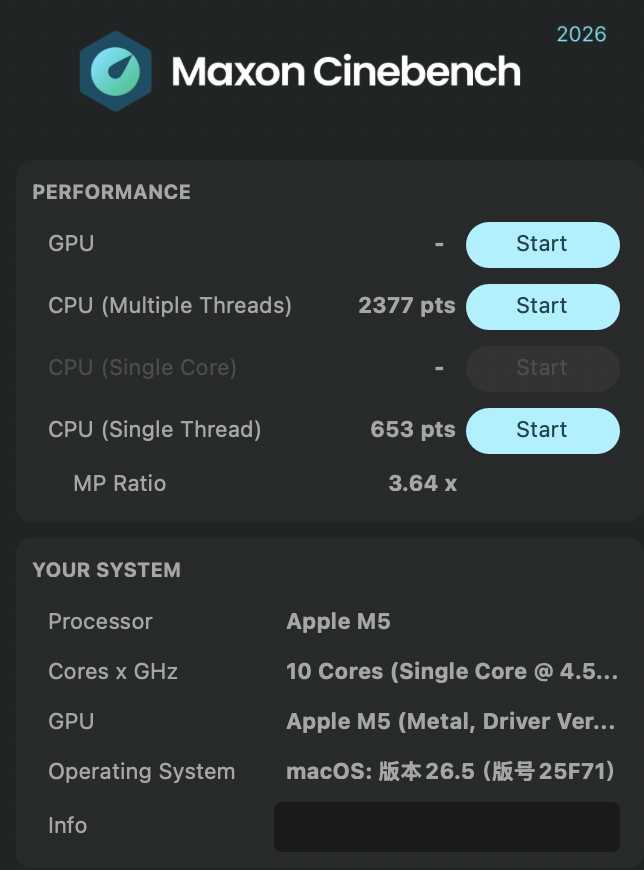
\includegraphics[width=\linewidth,height=6cm,keepaspectratio]{images/cinebench_m5.png}
        \end{minipage}
    }
    \caption{Apple M5 的 Cinebench 2026.1.3 结果界面}
\end{figure}

\begin{figure}[H]
    \centering
    \fbox{%
        \begin{minipage}[c][6cm][c]{12cm}
            \centering
            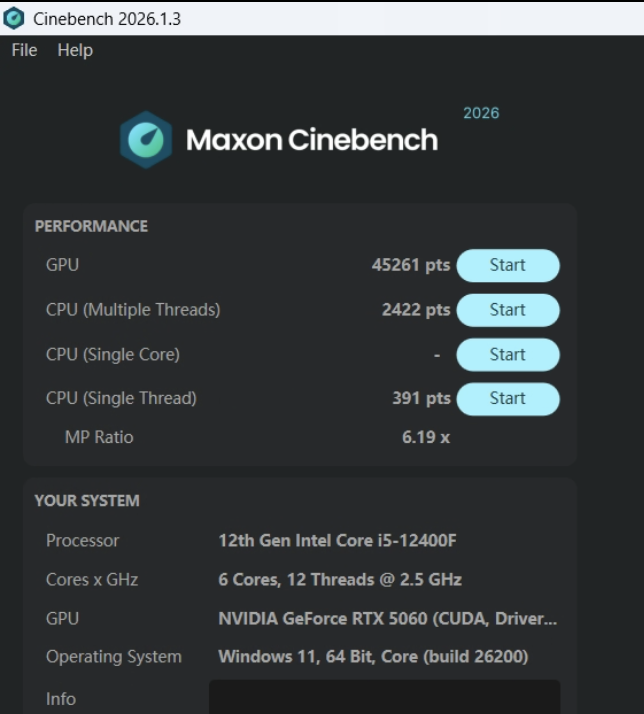
\includegraphics[width=\linewidth,height=6cm,keepaspectratio]{images/cinebench_i5_12400f.png}
        \end{minipage}
    }
    \caption{Intel Core i5-12400F 的 Cinebench 2026.1.3 结果界面}
\end{figure}

\section{性能差异的理论分析}

\subsection{CPU 性能公式与单线程差异}

CPU 执行时间可表示为：

\[
\mathrm{CPU\ Time}=\mathrm{Instruction\ Count}\times \mathrm{CPI}\times \mathrm{Clock\ Cycle\ Time}
=\frac{\mathrm{Instruction\ Count}\times \mathrm{CPI}}{\mathrm{Clock\ Rate}}
\]

对两个平台，可将时间比写为：

\[
\frac{T_{\mathrm{i5}}}{T_{M5}}
=\frac{IC_{\mathrm{i5}}}{IC_{M5}}
\times\frac{CPI_{\mathrm{i5}}}{CPI_{M5}}
\times\frac{f_{M5}}{f_{\mathrm{i5}}}
\]

相同 C++ 源代码、算法、输入和 workload 有助于控制实验变量，但 ARM64 与 x86-64 的指令序列不同，且两端使用 AppleClang 与 GNU 编译器，因此本实验没有直接测得 $IC$、$CPI$ 和实际运行频率，不能把时间差简单归结为“某一方主频更高”。例如，大规模普通矩阵乘法中 M5 的时间更短，说明这三个因素的综合结果更有利；快速排序中 M5 的稳定优势同样是比较、分支、访存和流水线共同作用的结果。

该公式也解释了 Cinebench 的现象：M5 单线程分数更高，表示其在该渲染 workload 的单线程综合执行效率更高；但是多线程分数还会叠加核心数量、线程资源、同步与共享资源竞争等因素，不能由单线程分数直接推出。

\subsection{阿姆达尔定律与多线程矩阵扩展}

阿姆达尔定律给出 $N$ 个并行执行单元下的理论加速比：

\[
S(N)=\frac{1}{(1-P)+\frac{P}{N}}
\]

其中，$P$ 是可并行部分在单线程测得工作量中的有效占比，$1-P$ 包含串行部分以及在实际测量中体现为不可并行开销的部分。这里的 $P$ 不是 CPU 的固定属性，也不是代码行数比例；它只描述本项目 $N=512$ 多线程矩阵乘法在特定平台和测试方式下的有效并行程度。

以 8 线程点估计，有：

\[
P=\frac{1-1/S}{1-1/N}
\]

\[
P_{M5}\approx\frac{1-1/5.128}{1-1/8}=0.920,
\qquad
P_{\mathrm{i5}}\approx\frac{1-1/6.858}{1-1/8}=0.976
\]

因此，在该矩阵 workload 中，i5-12400F 从自身单线程基线出发的相对扩展更接近线性；M5 的 8 线程加速比为 $5.128\times$，并行效率为 $64.1\%$，i5-12400F 则为 $6.858\times$ 和 $85.7\%$。不过，i5 的 12 线程实测加速比为 $8.551\times$，低于用 8 线程估计的理想预测 $9.511\times$，表明更多逻辑线程下的共享资源竞争、调度或同步开销开始增大。M5 的 10 线程实测加速比为 $5.646\times$，也低于理论线性加速。两端都体现出增加线程数不能无限线性提升性能。

这也帮助解释 Cinebench 的 MP Ratio：i5-12400F 的 $6.19\times$ 大于 M5 的 $3.64\times$，表示该渲染任务相对各自单线程基线的扩展幅度更大；它不推翻 M5 的较高单线程分数，更不等同于所有多线程应用中的绝对领先。

\subsection{核心/线程组织与存储局部性}

i5-12400F 具有 6 个物理性能核心和超线程形成的 12 个逻辑线程，逻辑线程并不等同于 12 个独立物理核心。M5 的测试环境报告为 10 个硬件并发线程，且采用性能核心与能效核心组成的异构设计。测试没有绑定核心，也没有读取硬件性能计数器，因此只能将这些结构差异作为解释线索，不能将某一个数值严格分配给特定核心或缓存层。

内存访问图显示，顺序访问通常保持较高且平稳的吞吐，体现了空间局部性和硬件预取的作用；随机访问随工作集增大明显下降，反映出访问局部性变差和更频繁的数据层次访问。M5 在大工作集随机访问下优势较大，是本测试实现、工作集和平台软件环境共同形成的结果；它并不构成对两种处理器缓存层级的直接测量或一般性结论。

\section{实验拓展应用：硬件选择讨论}

本实验不测试 GPU、磁盘、网络、能耗、整机价格或专业软件生态，因此硬件建议应限制在已测 CPU 工作负载范围内。

\begin{itemize}
\item 对于学生日常编程、脚本处理、轻量数据整理和以单线程响应为主的任务，M5 在 Cinebench 单线程以及本实验的快速排序、大规模筛法和大规模普通矩阵乘法中表现出较短执行时间，可作为移动学习与开发场景的有力选择。
\item 对于能够充分利用多线程的 CPU 渲染、编译或批处理任务，i5-12400F 的 Cinebench MP Ratio 和多线程矩阵相对扩展更高。若软件可稳定并行且台式机的散热、内存和供电配置合适，其并行扩展能力值得关注。
\item 对于随机访问密集、工作集较大的 CPU 数据处理任务，本项目中 M5 的吞吐优势较明显；但真实应用还受数据结构、编程语言、内存容量和后台负载影响，应使用目标软件复测后再作购买决定。
\item 对于视频剪辑、三维图形和游戏等强依赖 GPU 的应用，本报告没有 GPU 测试数据，不能据此评价显卡、游戏帧率或整机创作性能。Cinebench 的 CPU 渲染分数也不能替代 GPU 渲染测试。
\end{itemize}

\section{实验总结与体会}

本实验使用两个不同维度的系统性能评价方法：自建 Toy Benchmark 提供可控、可重复、可追溯的微观 workload 数据，Cinebench 2026 提供真实 CPU 渲染任务的补充观察。Toy Benchmark 的 10 次正式重复结果表明，M5 在大规模筛法、快速排序、大规模普通矩阵乘法、相同线程数的多线程矩阵乘法和多数大工作集内存访问中具有更短时间或更高吞吐；i5-12400F 则在小规模筛法、$N=256$ 单线程矩阵和部分小工作集内存访问中占优，并且在多线程矩阵和 Cinebench 渲染中体现出更高的相对扩展能力。

通过阿姆达尔定律可以看到，多线程性能取决于可并行比例和各类不可并行开销，而不是简单取决于线程数；通过 CPU 性能公式可以看到，执行时间由指令数、CPI 和频率共同决定，主频并非唯一解释。实际测试还使我认识到，实验结论必须区分绝对完成时间与相对加速比，区分 10 次统计结果与单次补充结果，并明确编译器、操作系统、核心调度和测试 workload 所带来的边界。

后续若需要提高 Cinebench 部分的统计可靠性，可在保持版本、系统状态和测试顺序一致的条件下增加重复次数；但不应修改本次已保存的 Toy Benchmark 原始数据。最终结论仅适用于本报告规定的源码、算法、输入、编译配置、操作系统和测试环境，不能泛化为“ARM 优于 x86”或“x86 优于 ARM”。

\section{附录：数据可追溯性与参考资料}

\subsection{数据与复现实验命令}

本实验的完整数据和绘图脚本均位于仓库 \url{https://github.com/Hanggoash/Lab1}。关键文件如下：

\begin{itemize}
\item M5 原始数据：\texttt{results/macos-arm64/raw/run\_20260914\_173637\_206.csv}。
\item M5 元数据：\texttt{results/macos-arm64/raw/metadata\_20260914\_173637\_206.json}。
\item i5-12400F 原始数据：\texttt{results/windows-x86\_64/raw/run\_20260914\_172225\_638.csv}。
\item i5-12400F 元数据：\texttt{results/windows-x86\_64/raw/metadata\_20260914\_172225\_638.json}。
\item 平台汇总：\texttt{results/macos-arm64/summary/summary.csv} 与 \texttt{results/windows-x86\_64/summary/summary.csv}。
\item 跨平台汇总：\texttt{results/comparison/summary/} 下按 benchmark 拆分的 CSV，以及 \texttt{overall\_comparison.csv}。
\item 图片：\texttt{results/comparison/figures/} 下的 7 张 PNG 图。
\end{itemize}

在两端 raw 数据均存在时，可在仓库根目录执行：

\begin{lstlisting}
python scripts/analyze.py
python scripts/plot.py
\end{lstlisting}

以上命令只读取 raw CSV，不修改原始数据；它们重新生成平台汇总、跨平台比较表和报告插图。Cinebench 两张截图应保存为 \texttt{images/cinebench\_m5.png} 与 \texttt{images/cinebench\_i5\_12400f.png}，以对应正文中的插图路径。

\subsection{参考资料}

\begin{enumerate}[label={\arabic*.}]
\item Apple. Apple unleashes M5, the next big leap in AI performance for Apple silicon. \url{https://www.apple.com/newsroom/2025/10/apple-unleashes-m5-the-next-big-leap-in-ai-performance-for-apple-silicon/}
\item Intel. Intel Core i5-12400F Processor Specifications. \url{https://www.intel.com/content/www/us/en/products/sku/134587/intel-core-i512400f-processor-18m-cache-up-to-4-40-ghz/specifications.html}
\item Maxon. Cinebench. \url{https://www.maxon.net/en/cinebench}
\item Amdahl, G. M. Validity of the Single Processor Approach to Achieving Large Scale Computing Capabilities. \textit{AFIPS Conference Proceedings}, 1967.
\end{enumerate}

\end{document}
